\documentclass[letterpaper, 10pt, conference]{ieeeconf}
\overrideIEEEmargins

% The following packages can be found on http:\\www.ctan.org
\usepackage{graphics} % for pdf, bitmapped graphics files
\usepackage{epsfig} % for postscript graphics files
%\usepackage{mathptmx} % assumes new font selection scheme installed
\usepackage{times} % assumes new font selection scheme installed
\usepackage{amsmath} % assumes amsmath package installed
\usepackage{amssymb} % assumes amsmath package installed
\usepackage[activate={true, nocompatibility}, final, tracking=true,
 kerning=true, spacing=true, factor=1000, stretch=20, shrink=20]{microtype} % nicer typesetting
\usepackage{booktabs}
\usepackage{tabularx}

\usepackage{fixmath}
\usepackage{array}
\usepackage{multirow}
\usepackage{bm}
\usepackage{mathrsfs}
\newcolumntype{C}{>{$}c<{$}}
\newcolumntype{R}{>{$}r<{$}}

\usepackage{lmodern}

%\newcommand{\matr}[1]{\bm{#1}}
%%\newcommand{\matr}[1]{#1}
\newcommand{\matr}[1]{\mathbold{#1}}
\newcommand{\graph}[1]{\mathcal{#1}}

\newcommand{\T}{\top}
\newcommand{\upto}{\mathinner {\ldotp \ldotp}}

\DeclareMathOperator*{\argmin}{arg\min}

\title{\LARGE \bf Portfolio Optimization Using Preference Relation Based on Statistical Arbitrage}
\author{Lovre Mr\v{c}ela et al.}

\begin{document}

  \maketitle
  \thispagestyle{empty}
  \pagestyle{empty}
    
  \begin{abstract}
    
  We propose a new algorithm for portfolio optimization based on statistical arbitrage, using potential method to obtain the most preferred assets.
  A graph that represents preference flow among financial assets (i.e. if an edge exists going from asset $\mathbold{A}$ to asset $\mathbold{B}$, then $\mathbold{A}$ is preferred over $\mathbold{B}$) is constructed at each time step, using a statistical arbitrage algorithm.
  Preference relation among the assets is imposed by the preference flow.
  Preference for each particular asset is then calculated using the potential method\cite{caklovic}, from which the most preferred assets are selected into the portfolio for each time step.
  
  Method has been tested on contiguous subset of shares from S\&P 500 index.
  Trading cost of 0.1\% is also included.
  Portfolios obtained by the algorithm yield annualized Sharpe ratios of over 1.0.
  Algorithm performs better when provided with a larger number of assets, as number pairs considered increases, providing more insight into the market behavior.
  
  \end{abstract}
  
  \section{INTRODUCTION}
  
%  The task of portfolio optimization is to try to enhance various criteria, which most of the time include maximization of expected return and minimization of deviation\dots
  
  Classical statistical arbitrage methods take into account a pair of assets whose prices behave similarly during certain period of time.
  Similarity is measured by cointegration, correlation, or some other measure in order to find a moment in time when those assets' prices exceed what was statistically determined as highly confident range.
  When such opportunities present themselves, we can take advantage by predicting that prices will return once again to the confident range in the next time step, and do the trading in accordance with this prediction.
  
  In this paper, we propose a new method based on those predictions that are obtained by the statistical arbitrage method, using statistical measures as a proxy for describing the preference relations between pairs of assets.
  Next, a graph is formed based on those relations, so that mutual interaction of assets might be analyzed.
  This graph imposes a preference relation among the assets that are included in it.
  Finally, assets are sorted by preference and included into the portfolio.
  The idea of this method is to create a generalization of statistical arbitrage methods that is more robust and performs better when working with a larger number of assets by trying to take into account mutual interaction of assets.
  
%  Each asset is compared to all other assets while looking for such specific deviations, so, in general, this algorithm performs better where there is larger number of assets.
  
  
%  Approach taken in this paper relies on statistical anomalies which are detected by observing past windows of time at each time step.
%  In this paper, approach was to create a portfolio using a large number of assets among which exist pairs that behave similarly during certain period.
%  At each time step, a past window of time is observed for finding pairs that abruptly stop behaving similarly.
  
  \section{CONCEPTS AND METHODS}
  
  Following are descriptions of the key components of the algorithm: outline of the preference relation and utility function, graph of preference flow, and potential method.
  
  \subsection{Preference relation and utility function}
  
  Let $\Omega$ be any set of entities.
  Preference relation $\succ$ defined over $\Omega \times \Omega$ is a strict weak ordering that describes the way humans prefer some entity over another.
  This relation is specific in that it is ($\forall x, y, z \in \Omega$):
  \begin{itemize}
    \item \textit{irreflexive}: every entity $x$ is not preferrable over itself, %($\neg \left( x \succ x \right)$),
    \item \textit{asymmetrical}: if $x$ is preferrable over some $y$, then $y$ is not preferrable over $x$, %($x \succ y \Rightarrow \neg \left( y \succ x \right)$),
    \item \textit{transitive}: if $x$ is preferrable over $y$, and $y$ is preferrable over $z$, then $x$ is also preferrable over $z$, %($x \succ y \wedge y \succ z \Rightarrow x \succ z$),
    \item \textit{transitive in incomparability} (noting that $x$ and $y$ may be \textit{incomparable}, i.e. neither $x$ is preferrable over $y$, nor $y$ is preferrable over $x$): if $x$ is incomparable with $y$, and $y$ is incomparable with $z$, then $x$ is also incomparable with $z$.
  \end{itemize}

  We naturally assume this kind of relation we describe relationships among the assets.
  Determining that some asset is preferred over another is easier than assigning a preference rank to each asset individually, especially for a larger number of assets.
  However, the latter is more useful for decision making, and therefore it is desirable to find a way of sorting assets in the order of preference.
  
  Utility function $U\colon \Omega \to \mathbb{R}$ is mapping from entities to real numbers, in such way that order of the mapping corresponds to the preference order of the entities, i.e. $\forall x, y \in \Omega, U(x) > U(y) \Rightarrow x \succ y$.
  One such mapping is obtained by using potential method that is described later in this paper.
  In addition to ordering of the entities, utility function also provides the intensity of preference for a particular entity, hence it is more informative when it comes to the decision making.
  
  \subsection{Graph of preference flow}
  
  Graph of preference flow is a weighted directed graph without multiple edges and loops, whose nodes represent entities, edges represent preference for one entity over another, and edge weights correspond to the strength of the preferences.
  If an edge between nodes is missing, it is considered that neither entity is preferable over another (incomparability of entities).
  The graph as a whole describes preference flow among the entities.
  An example of graph is shown on Fig. \ref{fig:graph}.
  
  \begin{figure}[h]
    \centering
    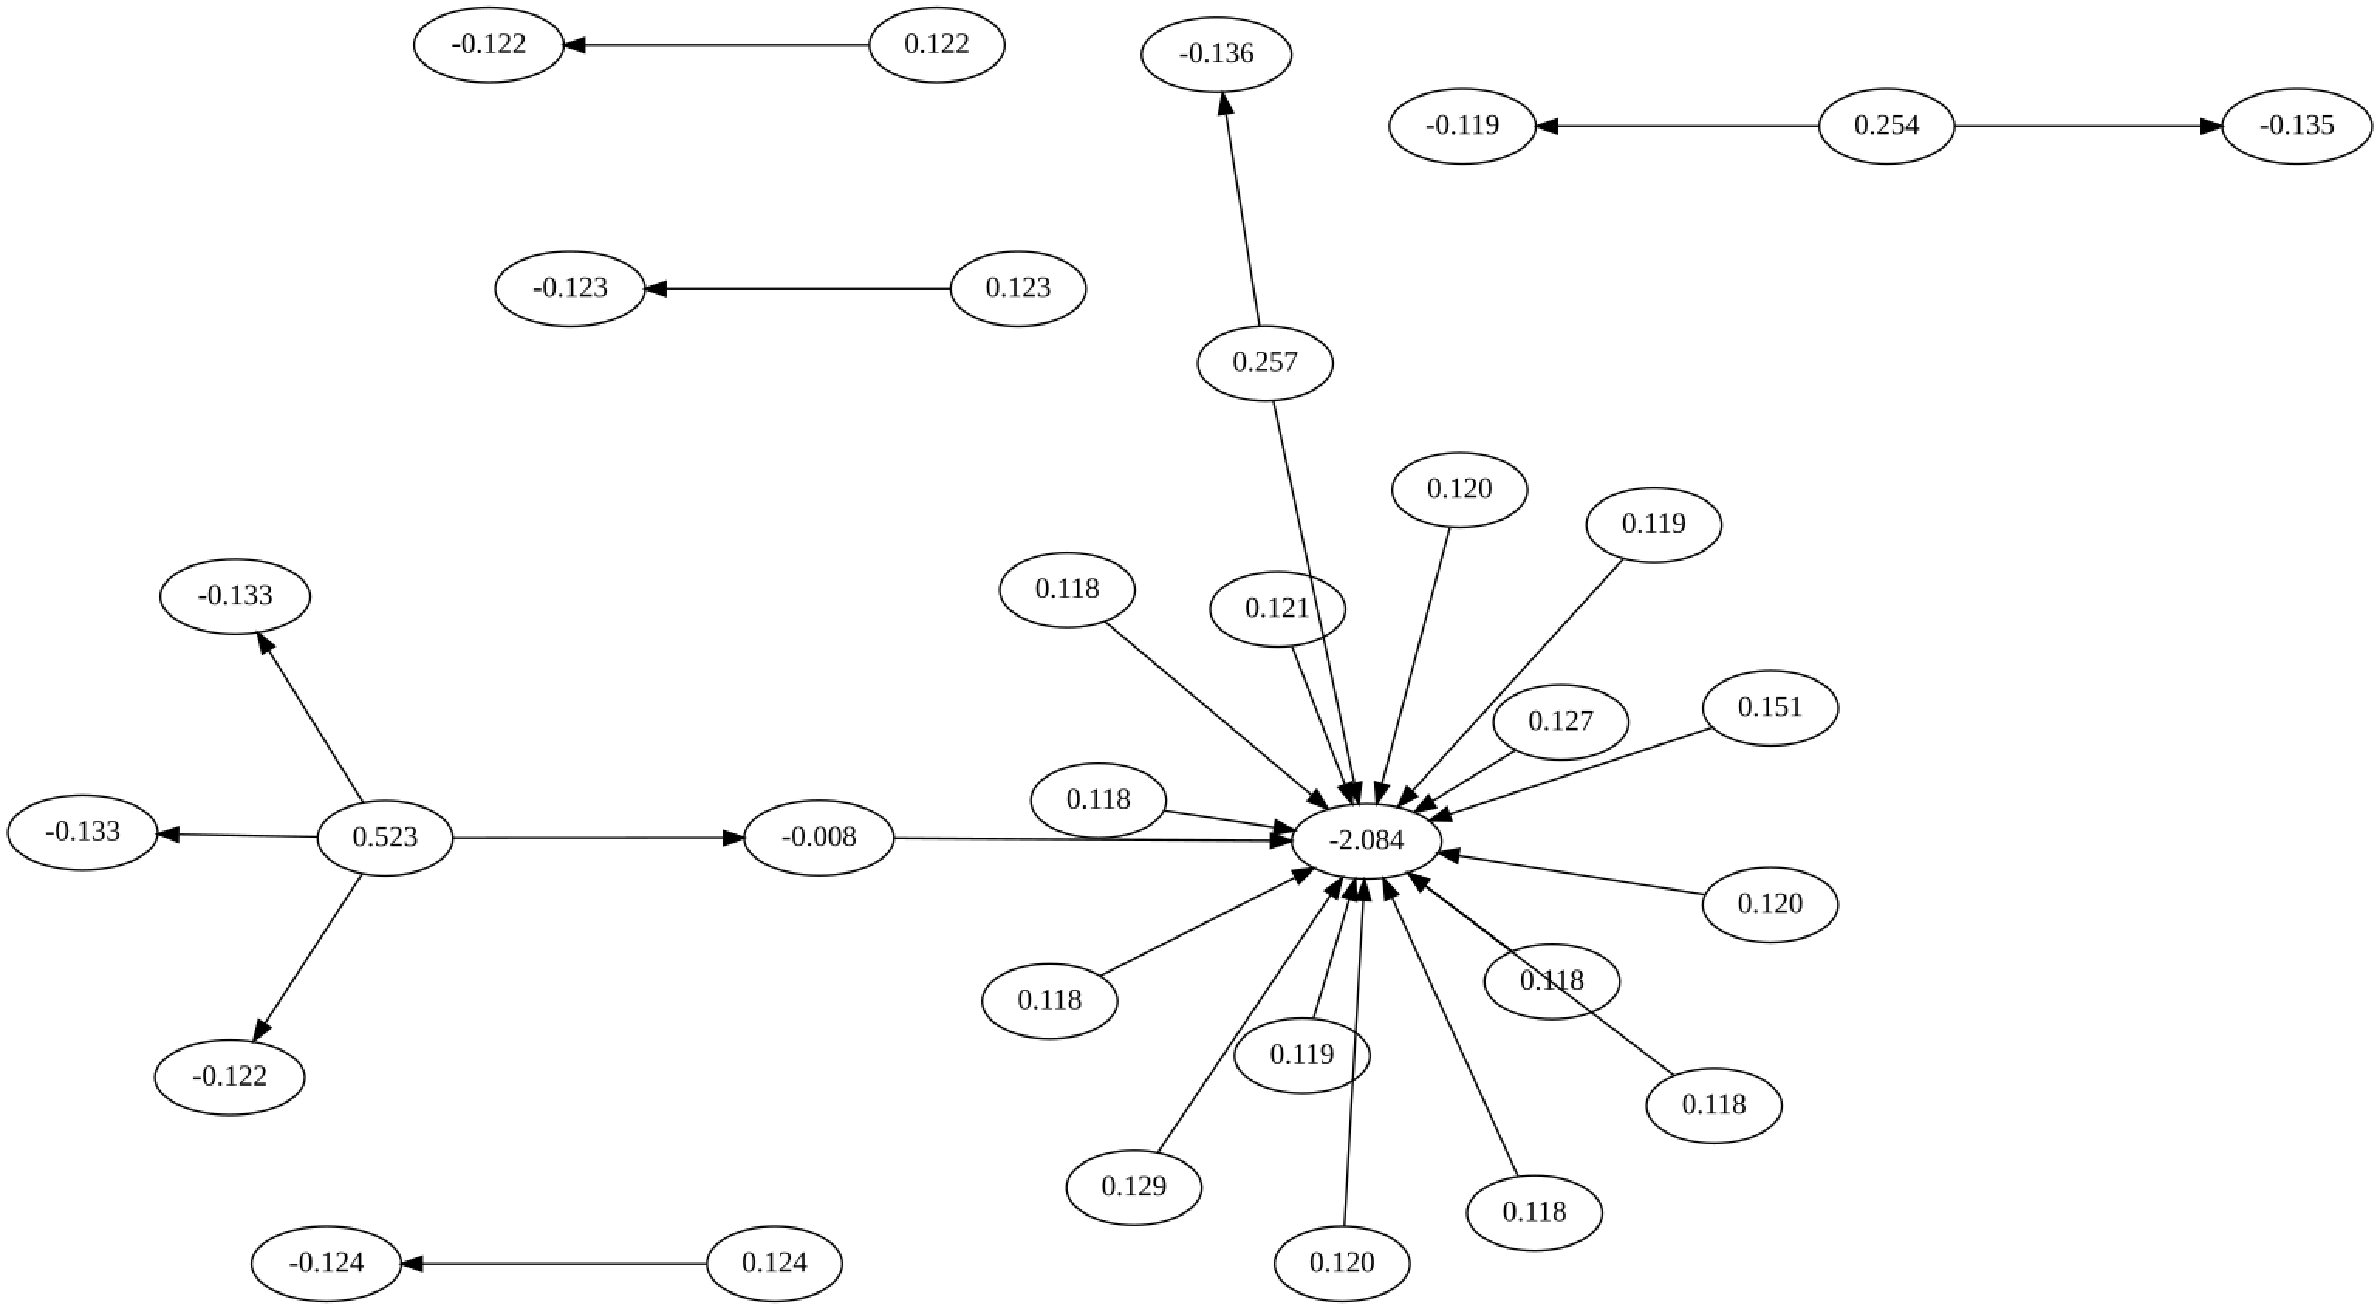
\includegraphics[width=\columnwidth]{graphics/graph.pdf}
    \caption{(TODO: put image with weights on edges) An example of a graph of preference flow. Asset number and calculated preference are inscribed in each node, and preference flows are shown on edges.}
    \label{fig:graph}
  \end{figure}

  Construction of the graph is based on a statistical arbitrage method.
  An edge going from node $i$ to node $j$ with weight $w_{i,j}$ will be present in the graph if and only if assets represented by nodes $i$ and $j$ have demonstrated similar behavior during the past period, but have suddenly diverged at the moment, as determined per statistical measures.
  Weight $w_{i,j}$ corresponds to the magnitude of this divergence.  
  A detailed description of used statistical measures the procedure is given later in \ref{sub:creating-graph}.
  
  Connections in this graph impose a preference relation among entities that are presented by the graph, in the way that an edge that goes from node $A$ to node $B$ means that $A$ is preferred over $B$.
  It is the case that neither node is in relation with itself (irreflexivity), and that no multiple connections are allowed between two nodes (implies asymmetry).
  However, problems arise with the aforementioned properties of transitivity, and transitivity in incomparability, which may not hold for an arbitrarily constructed instance of the graph.
  This imposed preference relation should preferably be in compliance with all the aforementioned properties, but when it comes to larger number of entities, it may become infeasible to construct a graph of such qualities directly.
  Instead of aiming at a consistent preference relation, we devise a consistency measure that describes similarity between the original graph and its nearest consistent reconstruction, and use it as an additional parameter in decision making.
  
%  The measure of this preference flow is determined by a statistical arbitrage method, and it corresponds to the magnitude of a pair of assets prices ratio going out of what is considered statistically confident range.
%  

  %Preference of a node itself corresponds to the difference between the amount of flow going in and out of it.
  
%  The main idea of preference flow is that preference for a particular node depends on amount of preference which flows in and out of it.
%  This allows for some kind of generalized statistical arbitrage over multiple assets at a time.
   
  \subsection{Potential method}
  \label{sub:potential}
  From previously obtained graph it is possible to tell which pair of assets has the highest preference flow.
  However, it is not yet possible to directly tell which are the most or least preferrable assets, or obtain the measure of preference for individual assets.
  To calculate preferences for each node in the graph, we use the potential method\cite{caklovic}.
  The potential of a node corresponds to difference in amount of flow going in and out of the node.
  
%  A concise summary of the method is as follows:
%  \begin{enumerate}
%    \item 
    For the observed graph $\graph{G}$, let there be a total of $N$ nodes, and maximum of $E = \binom{N}{2}$ edges, in case of a complete graph.
    If $\graph{G}$ is not complete, we complete it by adding edges to it with weight 0 (direction doesn't matter),
    thus forming a complete graph $\graph{G}$ with $\binom{N}{2}$ edges.
    % In our case, graphs will be incomplete for most of the time, but they may be \textsl{supplemented} (TODO: opposite of `reduced') to complete graphs, if we treat missing edges as edges of weight 0 (direction doesn't matter).
    
%    \item
    Let $\matr{B}$ be the $E \times N$ incidence matrix of $\graph{G}$.
%    $\matr{B}$ has following properties:
%    \begin{enumerate}
%      \item each row corresponds to an edge in the graph, and each column to a node,
%      \item for every edge in the graph going from node $i$ to node $j$, there is a corresponding row that has $-1$ and $1$ in columns that correspond to nodes $i$ and $j$ respectively,
%      \item the remainder of elements in the matrix are zeros.
%    \end{enumerate}
%
%    \item
    Let $\matr{f}$ be $E \times 1$ vector that contains edge weights (i.e. preference flows).
    Order of the edges must be the same as order of the edges in $\matr{B}$.
    As mentioned before, in place of missing edges we simply put 0.
%    
%    \item
    Let $\matr{\phi}$ be $N \times 1$ vector that contains potentials of each node, in order that is the same as order of the nodes in $\matr{B}$.
    
%    \item 
    Now, if $\graph{G}$ was consistent, then $\matr{B}$, $\matr{\phi}$, and $\matr{f}$ would satisfy the equation
    \begin{equation}
    \label{eq:flowformula}
    \matr{B} \matr{\phi} = \matr{f}.
    \end{equation}
    Equation (\ref{eq:flowformula}) states that the difference between potential of any two nodes should result in weight of the edge between them.
    This is possible only for consistent graphs, and most of the time our graphs will be inconsistent.
    In that case we try to find an approximate solution $\matr{\phi^*}$ that minimizes the square error:
    \begin{gather}
    \matr{\phi^*} = \argmin_{\matr{\phi}} \left\{ \left \lVert \matr{B} \matr{\phi} - \matr{f}\textsl{} \right \rVert ^ 2 \right\} \nonumber \\ 
    \Downarrow \nonumber \\
    \label{eq:derivative}
    \frac{\partial \left \lVert \matr{B} \matr{\phi^*} - \matr{f} \right \rVert ^ 2}{\partial \matr{\phi^*}} = \mathbf{0}.
    \end{gather}
    Solving (\ref{eq:derivative}) via commonly used techniques of matrix calculus brings us to the following equation:
    \begin{equation}
    \label{eq:flow}
    \matr{B}^\T \matr{B} \matr{\phi^*} = \matr{B}^\T \matr{f}.
    \end{equation}
    Equation (\ref{eq:flow}) determines $\matr{\phi^*}$ up to a constant (i.e. solution has one degree of freedom), so the following constraint is also included:
    \begin{equation}
    \label{eq:sumiszero}
    \matr{j}^\T \matr{\phi^*} = 0
    \end{equation}
    where $\matr{j}$ is vector of ones with same dimension as $\matr{\phi^*}$.
    This ensures an unique solution for which total amounts of positive and negative potential will be equal.
    
%    \item
    Joining the previous two equations together by adding (\ref{eq:sumiszero}) to each row in (\ref{eq:flow}) results in:
    \begin{align}
    \matr{B}^\T \matr{B} \matr{\phi^*} + \matr{J} \matr{\phi^*} &= \matr{B}^\T \matr{f} \nonumber \\
    \label{eq:joined}
    \left[\matr{B}^\T \matr{B} + \matr{J} \right] \matr{\phi^*} &= \matr{B}^\T \matr{f},
    \end{align}
    where $\matr{J}$ is a matrix of ones with same dimension as $\matr{B}^\T \matr{B}$.
    Finally, solving (\ref{eq:joined}) for $\matr{\phi^*}$ gives us:
    \begin{equation}
    \label{eq:final}
    \matr{\phi^*} = \left[\matr{B}^\T \matr{B} + \matr{J} \right]^{-1} \matr{B}^\T \matr{f}.
    \end{equation}
%    \item 
    Furthermore, the term $\left[ \matr{B}^\T \matr{B} + \matr{J} \right]^{-1}$ in (\ref{eq:final}) can be simplified to $\frac{1}{N} \matr{I}$ due to $\matr{B}^\T \matr{B}$ being the Laplace matrix of a complete graph; thus, we can simplify (\ref{eq:final}) some more:
    \begin{equation}
    \matr{\phi^*} = \frac{1}{N} \matr{B}^\T \matr{f},
    \end{equation}
    to get as computationally optimal expression as possible.
    
%    \item
    Afterwards, we can calculate the consistent reconstruction $\matr{f^*}$ of preference  flow by simply plugging back $\matr{\phi^*}$ into (\ref{eq:flowformula}):
    \begin{equation}
    \matr{f^*} = \matr{B} \matr{\phi^*}.
    \end{equation}
    The reconstructed preference flow $\matr{f^*}$ compared to the original preference flow $\matr{f}$ may even contain some new and/or lose some old edges.
    In addition, $\matr{B}$, $\matr{\phi^*}$, and $\matr{f^*}$ now describe a consistent graph $\graph{G}^*$.
    It is now possible to define a consistency measure $\kappa$ as follows:
    \begin{equation}
    \label{eq:consistency}
    \kappa = \frac{\left \lVert \matr{f^*} \right \rVert}{\left \lVert \matr{f} \right \rVert}.
    \end{equation}
    Equation (\ref{eq:consistency}) represents the cosine of the angle between $\matr{f}$ and $\matr{f^*}$ in the column space of matrix $\matr{B}$.
    Consistency measure $\kappa$ tells us how consistent graph $\graph{G}$ was, compared to the $\graph{G}^*$.
    $\kappa$ ranges from 0 to 1, with 0 meaning full inconsistency (virtually unreachable), and 1 meaning full consistency.
    
%  \end{enumerate}
  
  \section{ALGORITHM} 
  
  Let there be total of $N$ assets in $D$ days.
  Let price of asset $i$ at the time step $t$ be $a_i^{(t)}$, for $i \in {\left[1, 2, \ldots, N\right]}$ and $t \in {\left[0, 1, \ldots, D-1\right]}$.
  The log prices $b_i^{(t)}$, and log price differences $c_{i,j}^{(t)}$ between assets $i$ and $j$ are obtained as follows:
  \begin{equation} b_i^{(t)} = \log\left(a_i^{(t)}\right) \end{equation}
  \begin{equation} c_{i,j}^{(t)} = b_i^{(t)} - b_j^{(t)}, \end{equation}
  and rolling means $m_{i,j}^{(t)}$ and standard deviations $d_{i,j}^{(t)}$ of log price differences over the past time window of size $T$ are obtained as follows:
   
  \begin{equation}
    \label{eq:mean}
    m_{i,j}^{(t)} = \frac{1}{T}\sum_{\tau = t - T}^{t - 1} c_{i,j}^{(\tau)}
  \end{equation}
  \begin{equation}
    \label{eq:deviation}
    d_{i,j}^{(t)} = \sqrt{\frac{1}{T}\sum_{\tau=t - T}^{t - 1} \left(c_{i,j}^{(\tau)} - m_{i,j}^{(t)} \right)^2}.
  \end{equation}
  
  Note that in summation used in (\ref{eq:mean}, \ref{eq:deviation}) time step $t$ was intentionally excluded, therefore summation goes only to $t - 1$.
  We use these calculations as basis for creating the portfolio.
  
%  Note that period over which means and standard deviations of log price differences are calculated does not include time step $t$.
%  Also note that calculating them separately for each time step $t$ is rather computationally inefficient when dealing with rolling windows of data.
%  Therefore, it is advisable to use a rolling algorithm as described in the appendix.
%  On that note, $c_{i,j}^{(t)}$, $m_{i,j}^{(t)}$, and $d_{i,j}^{(t)}$ may be more efficiently stored if stored contiguously in memory as a matrix, using following coding scheme: a pair $(i, j)$, where $i < j$, should be encoded to $k$ as:
%  \begin{equation} k = N \cdot (i - 1) + j - 1 - \left. i \cdot (i + 1) \middle/ 2\right., \end{equation}
%  and decoded from $k$ as:
%  \begin{equation} i = \left\lfloor N + 1/2 - \sqrt{(N + 1/2)^2 - 2(N + k)} \right\rfloor, \end{equation}
%  \begin{equation} j = k + i \cdot \left.(i + 1) \middle/ 2\right. - N \cdot (i - 1) + 1. \end{equation}
%  An example of proposed coding is shown on figure \ref{fig:coding}.
%  
%  \begin{figure}[h]
%    \centering
%    \begin{tabular}{C|CCCCC}
%      i/j & 1 & 2 & 3 & 4 & 5 \\ \hline
%      1 & \cdot & 0 & 1 & 2 & 3 \\
%      2 & \cdot & \cdot & 4 & 5 & 6 \\
%      3 & \cdot & \cdot & \cdot & 7 & 8 \\
%      4 & \cdot & \cdot & \cdot & \cdot & 9 \\
%      5 & \cdot & \cdot & \cdot & \cdot & \cdot
%    \end{tabular}
%    \hspace{0.8cm}
%    \begin{tabular}{C|CC}
%    k & i & j \\ \hline
%    0 & 1 & 2 \\
%    1 & 1 & 3 \\
%    2 & 1 & 4 \\
%    3 & 1 & 5 \\
%    4 & 2 & 3 \\
%    5 & 2 & 4 \\
%    6 & 2 & 5 \\
%    7 & 3 & 4 \\
%    8 & 3 & 5 \\
%    9 & 4 & 5 \\
%    \end{tabular}
%    \caption{Example of the proposed coding scheme, for $N = 5$. A dot $(\cdot)$ indicates that that combination is not used.}
%    \label{fig:coding}
%  \end{figure}
  
  \subsection{Creating the graph of preference flow}
  \label{sub:creating-graph}
  Using the obtained $c_{i,j}^{(t)}$, $m_{i,j}^{(t)}$, and $d_{i,j}^{(t)}$ it is now possible to create a graph of preference flow among assets for each time step $t$.
  Considering one time step $t$, we find all such pairs of assets $(i,j)$ that satisfy:
  \begin{equation}
    \label{eq:thresh}
    \left| c_{i,j}^{(t)} - m_{i,j}^{(t)} \right| > \alpha \cdot d_{i,j}^{(t)},
  \end{equation}
  i.e. current log price difference is at least $\alpha$ deviations distant from mean value of the past time window.
  An illustration is shown on Fig. \ref{fig:devmag}.
%  Parameter $\alpha$ determines how many pairs of assets should constitute the graph at current time step.
  Afterwards, for each observed pair $(i,j)$ that exceeds the threshold we add into graph vertices $i$ and $j$, with a weighed edge of weight $w_{i,j}^{(t)}$ going from $i$ to $j$.
  Weight $w_{i,j}^{(t)}$ is obtained as:
  \begin{equation}
    \label{eq:weight}
    w_{i,j}^{(t)} = \left. \left(c_{i,j}^{(t)} - m_{i,j}^{(t)}\right) \middle/ d_{i,j}^{(t)} \right..
  \end{equation}
  
  Thus it is possible to create a graph of preference flow for each time step $t \in \left[T, T + 1, \ldots, D-1\right]$.
  At some time steps it is possible that the graph could be empty, if it is the case that no pair $(i,j)$ satisfies (\ref{eq:thresh}).
  Setting lower values for parameter $\alpha$ yields denser graphs, and setting $\alpha = 0$ always yields complete graphs.
  
  \begin{figure}[h]
    \centering
    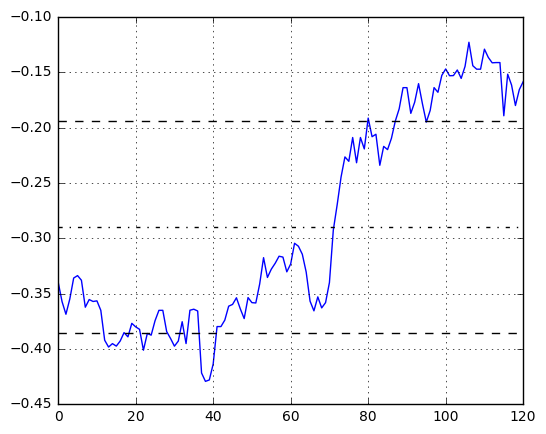
\includegraphics[width=0.9\columnwidth]{graphics/deviation-magnitude.png}
    \caption{Log price difference between a pair of assets $(i, j)$ during a period of $T + 1$ time steps, where $T = 120$.
    Dashed and dotted line represents mean value, and region between two dashed lines represents $\alpha$ standard deviation range from mean value, here $\alpha = 1$; both are calculated in the first $T$ time steps.
    During the time step $T + 1$, log price difference goes over $\alpha$ standard deviations above mean value of past period of size $T$.
    This would mean that two of the assets $i$ and $j$ would be added to the graph of preference flow at the time step $T + 1$.
    Weight $w_{i,j}$ describes current deviation from mean value.}
    \label{fig:devmag}
  \end{figure}
  
  \subsection{Choosing assets from graph}
  We obtain preference for each asset via the potential method, as described earlier in \ref{sub:potential}.
  By obtaining the measure of preference for each asset it is possible to pick assets for the portfolio.
  The most preferred assets should be bought while the least preferred should be short-sold if possible.
  
  Let $\matr{\phi}^{(t)} = \begin{bmatrix} \phi_1^{(t)} & \phi_2^{(t)} & \ldots & \phi_N^{(t)} \end{bmatrix}$ denote vector of preferences of assets at time step $t$ and $\phi_i^{(t)}$ denote the preference for asset $i$ at time step $t$.
  When picking the assets for the portfolio we take into consideration the consistency measure $\kappa$ as well.
  Lower values of $\kappa$ suggest that we should diversify our portfolio by including some more assets in the order of preference, while higher values suggest that it is safe to do trading with smaller number of assets.
  Portfolio diversification might be seen as a strategy for protection from fundamental risks, e.g. risk of asset default.
  
  The bound on the assets which will be taken into portfolio is proportional to the consistency measure $\kappa$.
  Depending on the nature of assets we may tune the consistency measure $\kappa$ to be more or less inclined to diversification by transforming it to $\kappa^\prime$:
  \begin{equation}
    \kappa^\prime = a + (1 - a)\kappa^b,
  \end{equation}
  where $a \in [0, 1], b \in \mathbb{R}^+$.
  For default values of $a = 0$, $b = 1$, $\kappa^\prime$ equals $\kappa$.
  
  For determining the assets that should be held in the portfolio at time step $t$, we find such assets $i$ for which holds:
  \begin{equation}
    \phi_i^{(t)} \ge \kappa^\prime \cdot \Phi,
  \end{equation}
  where $\Phi$ is $\max_j \left\{ \left| \phi_j \right| \right\}$.
  Likewise, for short-selling we choose those assets $i$ for which holds:
  \begin{equation}
    \phi_i^{(t)} \le -\kappa^\prime \cdot \Phi.
  \end{equation}
  For $a = 0$ diversification completely depends on consistency $\kappa$, while for $a = 1$ only the most preferred asset is held in the portfolio (no diversification).
  On the other hand, when $0 < b < 1$, algorithm is less inclined to diversification even when consistency is low, and when $b > 1$, algorithm is more inclined to diversification even when consistency is high. 
  
  \section{RESULTS}
  
  Results were obtained by testing on a set of 203 stocks that were contiguously included in S\&P 500 index from Jan 1st, 1980 thru Dec 31st, 2003, which includes 6261 trading days.
  A total of 20503 pairs of assets were probed for statistical arbitrage at each time step.
  Summary of results for various parameters is shown in the table \ref{table:results-1}.
  Best profit and Sharpe ratio has been achieved when using $\alpha = 0$.
  
  \begin{sidewaystable}[p]
  \centering
  \captionof{table}{Rezultati testiranja nad S\&P 203 skupu, uz $T = 60, \beta=0$.}
  \label{table:results-1}
  \begin{tabularx}{\hsize}{Xrrrrrrr}
    \toprule
    Parametar: & & & & & & & \\
    \quad a & \multicolumn{3}{c}{0.0} & \multicolumn{3}{c}{0.5} & \multicolumn{1}{c}{1.0} \\ \cmidrule(lr){2-4} \cmidrule(lr){5-7} \cmidrule(lr){8-8}
    \quad b & \multicolumn{1}{c}{0.5} & \multicolumn{1}{c}{1.0} & \multicolumn{1}{c}{2.0} & \multicolumn{1}{c}{0.5} & \multicolumn{1}{c}{1.0} & \multicolumn{1}{c}{2.0} & \multicolumn{1}{c}{/} \\ \midrule
    Prosječni povrat (godišnji) & 0.95339 & 0.88967 & 0.84463 & 0.98336 & 0.95663 & 0.89704 & 1.00223 \\
    Volatilnost (godišnja) & 0.77042 & 0.76595 & 0.74077 & 0.77905 & 0.77054 & 0.76660 & 0.78363 \\
    Sharpeov omjer (godišnji) & 1.23750 & 1.16152 & 1.14020 & 1.26225 & 1.24150 & 1.17015 & 1.27896 \\ \midrule
    Profit: &  &  &  &  &  &  &  \\
    \quad samo pozitivan & 89.27624 & 88.89440 & 88.32548 & 89.58775 & 89.29840 & 89.04414 & 89.55020 \\
    \quad samo negativan & -58.37779 & -59.03715 & -58.41396 & -58.24852 & -58.32385 & -59.02220 & -58.05316 \\
    \quad ukupan & 30.89846 & 29.85725 & 29.91152 & 31.33923 & 30.97456 & 30.02195 & 31.49704 \\
    \quad omjer pozitivnog i negativnog & 1.52928 & 1.50574 & 1.51206 & 1.53803 & 1.53108 & 1.50866 & 1.54256 \\ \midrule
    Prosječna točnost & 0.36485 & 0.39276 & 0.43413 & 0.34902 & 0.36458 & 0.39145 & 0.33241 \\
    Prosječni koeficijent obrtaja & 0.59976 & 0.64224 & 0.73597 & 0.57585 & 0.59947 & 0.64089 & 0.55112 \\ \midrule
    Stvarni profit, uz troškove trgovanja od 0.10\% & 23.46019 & 21.89215 & 20.78402 & 24.19757 & 23.53996 & 22.07361 & 24.66204 \\
    \bottomrule
  \end{tabularx}
\end{sidewaystable}

  \section{CONCLUSIONS}
  
  Algorithm works on pairs of assets, looking for those deviations which are uncommon, so generally it is expected to perform better where there is larger number of assets as more deviations will be discovered.
  It adapts to the inconsistence of preferences by picking variable number of assets into the portfolio.
    
  % \addtolength{\textheight}{-12cm} % This command serves to balance the column lengths
  % on the last page of the document manually. It shortens
  % the textheight of the last page by a suitable amount.
  % This command does not take effect until the next page
  % so it should come on the page before the last. Make
  % sure that you do not shorten the textheight too much.
  
  % \section*{APPENDIX}

  \begin{thebibliography}{9} % mind the label-width
    
  \bibitem{caklovic} L. \v{C}aklovi\'{c}, Decision Making by Potential Method
%    \bibitem{c2} W.-K. Chen, Linear Networks and Systems (Book style).	Belmont, CA: Wadsworth, 1993, pp. 123Ð135.
%    \bibitem{c3} H. Poor, An Introduction to Signal Detection and Estimation.   New York: Springer-Verlag, 1985, ch. 4.
%    \bibitem{c4} B. Smith, ÒAn approach to graphs of linear forms (Unpublished work style),Ó unpublished.
%    \bibitem{c5} E. H. Miller, ÒA note on reflector arrays (Periodical styleÑAccepted for publication),Ó IEEE Trans. Antennas Propagat., to be publised.
%    \bibitem{c6} J. Wang, ÒFundamentals of erbium-doped fiber amplifiers arrays (Periodical styleÑSubmitted for publication),Ó IEEE J. Quantum Electron., submitted for publication.
%    \bibitem{c7} C. J. Kaufman, Rocky Mountain Research Lab., Boulder, CO, private communication, May 1995.
%    \bibitem{c8} Y. Yorozu, M. Hirano, K. Oka, and Y. Tagawa, ÒElectron spectroscopy studies on magneto-optical media and plastic substrate interfaces(Translation Journals style),Ó IEEE Transl. J. Magn.Jpn., vol. 2, Aug. 1987, pp. 740Ð741 [Dig. 9th Annu. Conf. Magnetics Japan, 1982, p. 301].
%    \bibitem{c9} M. Young, The Techincal Writers Handbook.  Mill Valley, CA: University Science, 1989.
%    \bibitem{c10} J. U. Duncombe, ÒInfrared navigationÑPart I: An assessment of feasibility (Periodical style),Ó IEEE Trans. Electron Devices, vol. ED-11, pp. 34Ð39, Jan. 1959.
%    \bibitem{c11} S. Chen, B. Mulgrew, and P. M. Grant, ÒA clustering technique for digital communications channel equalization using radial basis function networks,Ó IEEE Trans. Neural Networks, vol. 4, pp. 570Ð578, July 1993.
%    \bibitem{c12} R. W. Lucky, ÒAutomatic equalization for digital communication,Ó Bell Syst. Tech. J., vol. 44, no. 4, pp. 547Ð588, Apr. 1965.
%    \bibitem{c13} S. P. Bingulac, ÒOn the compatibility of adaptive controllers (Published Conference Proceedings style),Ó in Proc. 4th Annu. Allerton Conf. Circuits and Systems Theory, New York, 1994, pp. 8Ð16.
%    \bibitem{c14} G. R. Faulhaber, ÒDesign of service systems with priority reservation,Ó in Conf. Rec. 1995 IEEE Int. Conf. Communications, pp. 3Ð8.
%    \bibitem{c15} W. D. Doyle, ÒMagnetization reversal in films with biaxial anisotropy,Ó in 1987 Proc. INTERMAG Conf., pp. 2.2-1Ð2.2-6.
%    \bibitem{c16} G. W. Juette and L. E. Zeffanella, ÒRadio noise currents n short sections on bundle conductors (Presented Conference Paper style),Ó presented at the IEEE Summer power Meeting, Dallas, TX, June 22Ð27, 1990, Paper 90 SM 690-0 PWRS.
%    \bibitem{c17} J. G. Kreifeldt, ÒAn analysis of surface-detected EMG as an amplitude-modulated noise,Ó presented at the 1989 Int. Conf. Medicine and Biological Engineering, Chicago, IL.
%    \bibitem{c18} J. Williams, ÒNarrow-band analyzer (Thesis or Dissertation style),Ó Ph.D. dissertation, Dept. Elect. Eng., Harvard Univ., Cambridge, MA, 1993. 
%    \bibitem{c19} N. Kawasaki, ÒParametric study of thermal and chemical nonequilibrium nozzle flow,Ó M.S. thesis, Dept. Electron. Eng., Osaka Univ., Osaka, Japan, 1993.
%    \bibitem{c20} J. P. Wilkinson, ÒNonlinear resonant circuit devicesize (Patent style),Ó U.S. Patent 3 624 12, July 16, 1990. 

  \end{thebibliography}
\end{document}
